\documentclass[a4paper,10pt]{article}
\usepackage[utf8x]{inputenc}

%\usepackage{natbib}

\usepackage{amssymb, amsmath}
\usepackage{mathtools}
%\usepackage{amsthm} % For teoremer,

\DeclareMathOperator*{\argmax}{arg\,max}

\usepackage{comment}
\usepackage{tabularx}
\usepackage{listings}

\setlength{\parskip}{\bigskipamount}
\setlength{\parindent}{0pt}

%\usepackage{caption}
%\usepackage{subcaption}

\usepackage{color}
\usepackage{xcolor}
\definecolor{solarbg}{HTML}{FDF6E3}

\usepackage[hidelinks]{hyperref}

%opening
\title{TMA4280|Introduction to Supercomputing\\
  Exercise 6}
\author{Caroline Anne Sæhle, Christer Emil Haga Bru, Jean Niklas L'orange\\
Department of Computer and Information Science\\
Norwegian University of Science and Technology
}
\date{\today}

\begin{document}
\lstset{language=C, frame=single}

\maketitle
\thispagestyle{empty}
\addtocounter{page}{-1}
\newpage

\section{Introduction}

This exercise asks us to solve the two-dimensional Poisson problem by
implementing a parallel program with MPI and OpenMP. We will look at different
approaches and ways to improve performance, and compare them with a sequential
variant.


\section{The Poisson Problem}

Poisson's equation is defined as

\begin{align}
  - \nabla ^2 u &= f &\text{in~} \Omega \\
  u &= 0 &\text{on~} \partial\Omega
\end{align}
where $\nabla^2$ is the Laplacian, the second order differential
operator. {\em u} and {\em f} are both real- or complex-valued functions on a
manifold, in our case the Euclidian space.

We discretize this problem on a uniform, finite, difference grid with a mesh
spacing $h = 1/n$. To obtain the second derivative, one approximate $u$ by using
the 5-point stencil. The problem can thus be expressed as

\begin{equation}
  -\cfrac{u_{i+1, j} + u_{i, j+1} +u_{i-1, j} +u_{i, j-1} - 4u_{i, j}}{h^2} =
  f_{i,j}
\end{equation}

where $f_{i,j} = f(x_i, y_j)$ and $u_{i,j} \approx u(x_i, y_j)$, the
approximation.

Now, our problem is reduced to find a solution to

\begin{equation}
  \underline A \underline u = \underline f
\end{equation}

where $\underline A$ represents the discrete Laplace operator, $\underline u$ is
a vector representing the unknowns, and $\underline f$ is a known right hand
side vector.

Now, let $\underline T = \underline A$, and let $\underline U$ be a matrix with
the same size as $\underline T$. By expressing the partial derivatives of both
$x$ and $y$ with $\underline T$ and $\underline U$, we can solve this problem as
a system of equation. Thus, let

\begin{align}
  \cfrac{1}{h^2}(\underline{TU})i,j \simeq& -(\cfrac{\partial^2u}{\partial x^2})i,j \\
  \cfrac{1}{h^2}(\underline{UT})i,j \simeq& -(\cfrac{\partial^2u}{\partial y^2})i,j
\end{align}

and express Equation 1 through $\underline T$ and $\underline U$ as follows:

\begin{equation}
  (\underline{TU} + \underline{UT})i,j = h^2f_{i,j} = \underline{G}
\end{equation}

Henceforth, our goal is now to solve

\begin{equation}
  \underline{TU} + \underline{UT} = \underline G
\end{equation}

where $\underline T$, $\underline U$, $\underline G \in \mathbb{M}_{M\times M}$.

\subsection{Diagonalization}

We thus have to find the eigenvalues and the orthonormal eigenvectors to
$\underline T$ and place them into $\underline Q$, an orthonormal matrix. As
$\underline Q$ represent all the orthonormal eigenvectors, we have that

\begin{equation}
  \underline T = \underline Q \underline \Lambda \underline Q^T
\end{equation}
where $\underline \Lambda$ is the diagonal matrix with all the eigenvalues to
$\underline T$.

By combining Equation 8 and 9, we get
\begin{align}
  \underline {Q \Lambda Q^T U} + \underline {U Q \Lambda Q^T} &= \underline G \\
  \underline {\Lambda Q^T U Q} + \underline {Q^T U Q \Lambda} &= \underline{Q^T
    G Q} \\
  \underline {\Lambda \tilde{U}} + \underline {\tilde{U} \Lambda} &= \underline{\tilde{G}}
\end{align}

where
\begin{equation}
  \underline U = \underline{Q^T \tilde{U} Q}
\end{equation}

Out from this, we can now start on different method solving this issue.

\subsection{Methods}

The first we need to do, is to compute $\underline{\tilde{G}} = \underline Q^T
(h^2 \underline F) \underline Q$, which is essentially two matrix
multiplications as all these variables can be found. This will take
$\mathcal{O}(n^3)$ operations\footnote{Or $n^{\log_2 1 + o(1)}$, when using
  the Strassen algorithm.}.

The next we need to find is $\underline{\tilde{U}}$. From Equation 12, this is
trivial:

\begin{align*}
  \underline {\Lambda \tilde{U}} + \underline {\tilde{U} \Lambda} &=
  \underline{\tilde{G}}\\
  \lambda_i\tilde{u}_{i,j} + \lambda_j\tilde{u}_{i,j} &= \tilde{g}_{i,j} \\
  (\lambda_i + \lambda_j)\tilde{u}_{i,j} &= \tilde{g}_{i,j} \\
  \tilde{u}_{i,j} &= \cfrac{\tilde{g}_{i,j}}{\lambda_i + \lambda_j}
\end{align*}

It then follows that finding $\underline{\tilde{U}}$ can be done in
$\mathcal{O}(n^2)$ time.

Finding the original $\underline U$ is trivial by using Equation 13, which uses
$\mathcal{O}(n^3)$ time. When this calculation is done, we have thus solved the
Poisson problem in $\mathcal{O}(n^3)$ time.

\subsection{Improvements}

The implementation used in this exercise runs in $\mathcal{O}(n^2\log (n))$,
which is faster than the $\mathcal{O}(n^3)$ solution described above. To avoid
repeatability, a good explanation on how this solution works is explained in
great detail in ``{\em The Poisson Problem in $\mathbb{R}^2$: Fast
  Diagonalization Methods}'' (Einar M. Rønquist, 2011) and the reader is
encouraged to read this paper.

A very brief explanation of this implementation is that we look at how the
matrix multiplication is done. A matrix multiplication $\underline A \times
\underline B$ can be interpreted as a matrix $\underline A$ multiplied with $n$
vectors $\underline b_i$, which has the complexity $\mathcal{O}(n~n^2)$.
However, for each matrix multiplication $\underline A \underline b_i$, we can,
by using some assumptions, use the discrete sine transform to perform the
multiplication. As a discrete sine transform is using $\mathcal{O}(n \log (n))$
time, the total time is thus $\mathcal{O}(n^2\log (n))$ instead of the original
$\mathcal{O}(n^3)$.


\section{The Implementation}

The parallel implementation lies within {\tt parallel.c}. Most of this should be
relatively straightforward for people with basic knowledge in OpenMP and MPI,
but a small description of the changes from the original program will be given.

For single for loops, the single loop is prepended with a pragma, and an
eventual {\tt omp\_id} is defined inside. The id is used whenever multiple {\tt
  z} buffers are needed, and we don't want to allocate and free buffers if we
can avoid so. Henceforth, we make an array of buffers, and as such, {\tt z} is
a {\tt Real**} instead. The listing below is an example of such a setup.

\begin{lstlisting}
#pragma omp parallel for private(omp_id)
for (i=0; i < mpi_work; i++) {
  omp_id = omp_get_thread_num();
  fst_(b[j], &n, z[omp_id], &nn);
}
\end{lstlisting}

For double for loops, we only ensure that the inner loop's iterator is private,
and add this variable inside the private declaration in the OpenMP pragma.

As for the OpenMP reduction, we perform a local reduction through a specialized
OpenMp implementation, and send the result of the local reduction to a global
MPI reduction. The result is stored within the node with rank 0, and is printed
out afterwards.

\subsection{Transpose}

Instead of using \verb|MPI_Alltoallv|, we ended up using \verb|MPI_Alltoall|.
This requires repetitive calls to {\tt Alltoall}, so at first one may assume
that this may be slower than using {\tt Alltoallv}. However, the speed may be
roughly the same, and it may not be unrealistic that {\tt Alltoall} is faster
than {\tt Alltoallv}. This is because {\tt Alltoall} is easier for MPI to
optimize, whereas it is outright hard to optimize {\tt Alltoallv} as it has a
vast amount of configuration possibilities.

\begin{figure}[h]
  \centering
  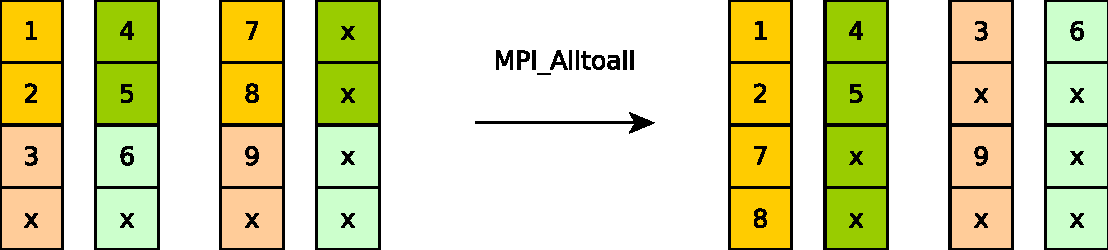
\includegraphics[width=0.8\textwidth]{img/transpose-1.pdf}
  \caption{The result of performing {\tt MPI\_Alltoallv} in the implementation.}
  \label{fig:t1}
\end{figure}

We then perform a local transponation. This works as follows: We perform a local
transponation on each square block we store in memory. The square block's size
has the amount of rows each node contains multiplied with the amount of nodes.
Consequently, each row may be a bit larger than the original $m$, with the
result of a simpler transpose implementation which may be potentially faster
than using {\tt Alltoallv}.

\begin{figure}[h]
  \centering
  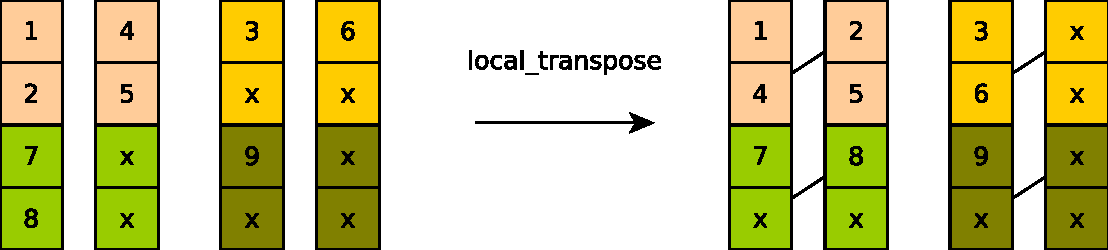
\includegraphics[width=0.8\textwidth]{img/transpose-2.pdf}
  \caption{Performing {\tt local\_transpose} in the implementation.}
  \label{fig:t2}
\end{figure}

In order to load balance as much as possible, the last node will potentially do
less work than the other nodes, compared to the other scenario where it has to
perform more work. Both Figure \ref{fig:t1} and \ref{fig:t2} shows the edge case
where the last node has not as many rows to work with as the previous nodes.

\section{Results}

\begin{table}[h]
   \centering
    \begin{tabular}{| l | l | l | l | l | l | l |}
    \hline
    \bf{n} & \bf{Nodes} & \bf{Processes} &\bf{Threads} & \bf{Average time} & \bf{Average }$S_{p}$ & \bf{Efficiency} \\ \hline
    	16384 & 1 & 1 & 1 & 788.65s & 1 & 1 \\ \hline
	16384 & 3 & 3 & 12 & 45.91s & 17.18 & 0.48 \\ \hline
	16384 & 3 & 12 & 3 & 33.80s & 23.33 & 0.65 \\ \hline
	16384 & 3 & 36 & 1 & 31.11s & 25.35 & 0.70  \\ \hline
	16384 & 1 & 1 & 12 & 86.47s & 9.12 & 0.75 \\ \hline
	16384 & 1 & 6 & 2 & 69.57s & 11.33 & 0.94 \\ \hline
	16384 & 3 & 18 & 2 & 32.75s & 24.08 & 0.67 \\ \hline
	16384 & 3 & 36 & 1 & 31.17s & 25.30 & 0.70\\ \hline
    \end{tabular}
\end{table}

\begin{table}[h]
   \centering
    \begin{tabular}{| l | l | l | l | l | l | l |}
    \hline
    \bf{n} & \bf{Nodes} & \bf{Processes} &\bf{Threads} & \bf{Average time} & \bf{Average }$S_{p}$ & \bf{Efficiency} \\ \hline
	4096 & 1 & 1 & 1 & 42.65s & 1 & 1 \\ \hline
	4096 & 3 & 36 & 1 & 2.93s & 14.56 & 0.40 \\ \hline
	4096 & 3 & 18 & 2 & 2.84s & 15.02 & 0.42 \\ \hline
	4096 & 1 & 6 & 2 & 4.80s & 8.89 & 0.74 \\ \hline
	4096 & 1 & 1 & 12 & 5.49s & 7.77 & 0.65  \\ \hline
    \end{tabular}
\end{table}

\end{document}
